
\subsection{Identity-Transformation Algorithms}
\label{subsec:overview}

We design identity-transformation algorithms,
   %  $\mathcal{F}_{PID_{RP}}$, $\mathcal{F}_{PID_{U}}$ and $\mathcal{F}_{Acct}$,
    on an elliptic curve $\mathbb{E}$.
Table \ref{tbl:notations-protocol} lists the notations,
    and the subscript $j$ and/or the superscript $i$ may be omitted in the case of no ambiguity.

\begin{table}[tb]
\footnotesize
    \caption{The notations in the UPPRESSO protocols}
    \centering
%    \begin{tabular}{|c|c|c|}
    \begin{tabular}{|p{1.0cm}|p{6.60cm}|} \hline
    {\textbf{Notation}} & {\textbf{Description}} \\ \hline
    {$\mathbb{E}$, $G$, $n$} & {$\mathbb{E}$ is an elliptic curve over a finite field $\mathbb{F}_q$. $G$ is a base point (or generator) of $\mathbb{E}$, and the order of $G$ is a prime number $n$.} \\ \hline
    {$ID_U$} & {$ID_U = u \in [1, n)$, is the user's unique identity at the IdP; \textcolor{blue}{$u$ is kept unknown to RPs.}} \\ \hline
   {$ID_{RP_j}$} & {$ID_{RP} = [r]G$, is the $j$-th RP's unique identity, publicly known, where $r \in [1, n)$, \textcolor{blue}{is known to only the IdP.}} \\ \hline
    {$t$} & {$t \in [1, n)$, is a user-generated random integer in a login instance; \textcolor{blue}{$t$ is kept secret to the IdP.}} \\ \hline
    {$PID_{RP_j}^i$} & {$PID_{RP} = [t]{ID_{RP}} = [tr]G$, is the $j$-th RP's pseudo-identity, in the user's $i$-th login instance to this RP.} \\ \hline
    {$PID_{U,j}^i$} & {$PID_U = [{ID_U}]{PID_{RP}} = [utr]G$, is the user's pseudo-identity, in the user's $i$-th login instance to the $j$-th RP.} \\ \hline
     {$Acct_j$} & {$Acct = [t^{-1}\bmod n]PID_{U} = [ID_U]ID_{RP} = [ur]G$, is the user's account at the $j$-th RP.} \\ \hline
    {$SK$, $PK$} & {The IdP's key pair, a private key and a public key, to sign and verify identity tokens and RP certificates.} \\ \hline
%    {$T$} & {The trapdoor to derive $Account$: $T=N_U^{-1} \bmod n$.} \\ \hline
    {$Enpt_{RP_j}$} & {The $j$-th RP's endpoint, to receive the identity tokens.} \\ \hline
    {$Cert_{RP_j}$} & {A signed RP certificate binding $ID_{RP_j}$ and $Enpt_{RP_j}$.} \\ \hline
%    {$PEnpt_{U,j}^i$} & {A user-generated random "pseudo-endpoint'', in the user's $i$-th login instance to the $j$-th RP.} \\ \hline
    \end{tabular}
    \label{tbl:notations-protocol}
\end{table}


For a user,
           a unique random integer $u$ is assigned by the IdP (i.e., $ID_U = u$).
When an RP is registering,
            the IdP generates a random number $r$, and $ID_{RP} = [r]G$, a unique point on $\mathbb{E}$, is assigned.
Here,
%$u, r \in [1,n)$, %$r$ is unknown to the RP, and
 $[r]G$ is the addition of $G$ on the curve $r$ times.

\vspace{0.5mm}
\noindent {\bf $\boldsymbol{ID_{\boldsymbol{RP}}}$-$\boldsymbol{PID_{\boldsymbol{RP}}}$ Transformation.} A user selects a random number $t \in [1, n)$, as the trapdoor
         and calculates $PID_{RP}$.
\begin{equation}
PID_{RP} = \mathcal{F}_{PID_{RP}}(ID_{RP}) = [t]{ID_{RP}} = [tr]G
\label{equ:PIDRP}
\end{equation}
\noindent {\bf $\boldsymbol{ID_U}$-$\boldsymbol{PID_U}$ Transformation.}
On receiving an identity-token request with $ID_U$ and $PID_{RP}$,
    the IdP calculates $PID_{U}$.
\begin{equation}
PID_{U} = \mathcal{F}_{PID_U}(ID_U, PID_{RP}) =
  [{ID_U}]{PID_{RP}} = [utr]G
 \label{equ:PIDU}
\end{equation}


\noindent {\bf $\boldsymbol{PID_U}$-$\boldsymbol{Acct}$ Transformation.}
The trapdoor $t$ is sent to the target RP,
which then checks that $PID_{RP}$ enclosed in identity tokens is equal to $[t]ID_{RP}$.
After verifying a token binding $PID_U$ and $PID_{RP}$,
    it calculates $Acct$ as below.
\begin{equation}
Acct = \mathcal{F}_{Acct}(PID_{U})
   = [t^{-1} \bmod n]PID_{U}
   \label{equ:Account}
\end{equation}

From Equations \ref{equ:PIDRP}, \ref{equ:PIDU} and \ref{equ:Account}, it is derived that
\begin{equation*}
   Acct =  [t^{-1}utr \bmod n]G = [ur]G = [ID_U]ID_{RP}
   \label{equ:AccountNotChanged}
\end{equation*}
The RP derives an \emph{identical permanent} account from the identity tokens in different login instances,
    with the help of $t$. %from the user.
Given a user, the accounts at different RPs are inherently unique;
while, given an RP, the accounts of different users are also unique.
It is impossible for the RP to derive $ID_U$ from either $PID_U$ or $Acct$ due to the elliptic curve discrete logarithm problem (ECDLP).
Because $t$ is random in $\mathbb{Z}_n$ and unknown to the IdP,
from the IdP's view,
    $PID_{RP}$ is indistinguishable from a random variable on $\mathbb{E}$,
    and the IdP learns nothing about $ID_{RP}$ from $PID_{RP}$.
%Section \ref{sec:analysis} presents more detailed analyses.

Note that $r$ is kept secret to the RP; otherwise, two colluding RPs with $ID_{RP_j} = [r]G$ and $ID_{RP_{j'}} = [r']G$ could link a user's accounts by checking whether $[r']Acct_j = [r]Acct_{j'}$ or not.

\textcolor{blue}{$PID_{RP} = [t]ID_{RP}$ is negotiated between a user and an RP,
    while $t$ is a random number known only to them.
The user and the RP need to calculate $PID_{RP}$ independently; or, more exactly,
 one computes $PID_{RP} = [t]ID_{RP}$, and the other checks whether $PID_{RP}$ is equal to $[t]ID_{RP}$ or not.
In the above descriptions,
    the user generates $t$, calculates $PID_{RP} = [t]ID_{RP}$ and sends $t$ to the RP.
After receiving $t$ from the user and extracting $PID_{RP}$ from a token,
    the RP checks that $PID_{RP} = [t]ID_{RP}$,
        because the correct account $[ID_U]ID_{RP}$ is derived \emph{only if} this equation holds (i.e., $PID_{RP} = [t]ID_{RP}$);
        otherwise, attacks happen as below.
To login as any $Acct$,
        a malicious user with $ID_{U'} = u'$ might generate a random number $t'$,
            and calculate $[t'u'^{-1}]Acct$ as $PID_{RP}$ to request an identity token.
Then, the IdP will calculate $PID_{U'} = [u'][t'u'^{-1}]Acct = [t']Acct$.
Without checking $PID_{RP} = [t']ID_{RP}$ or not,
        the RP will finally allow the malicious user to login as $[t'^{-1}]PID_{U'} = Acct$.}


\textcolor{blue}{Meanwhile,
    if the RP generates $t$, calculates $PID_{RP}$ and sends $t$,
the user still needs to by himself check that $PID_{RP} = [t]ID_{RP}$;
    otherwise, attacks happen as below.
A malicious user $U'$ initiates a login request to an honest RP,
    and receives $PID_{RP}$ from this RP.
Then $U'$ colludes with a malicious RP denoted as $RP'$,
    which intentionally sends $PID_{RP}$ to an honest user $U$ in some login instance.
Without checking $PID_{RP} = [t']ID_{RP'}$ or not,
    this honest user will present a token binding $PID_U$ and $PID_{RP}$ to $RP'$.
Finally, this token enables malicious $U'$ to login as the honest user's account at the honest RP.}
%In other words, this checking ensures RP designation,
%    because it is impossible to find $t$ and $t'$ satisfying that
%    $[t]ID_{RP} = [t']ID_{RP'}$,
%        when $ID_{RP} = [r]G$, $ID_{RP'} = [r']G$, but $r$ and $r'$ are unknown.
%See Section \ref{sec:analysis} for the detailed proofs of security and privacy.



\subsection{The Designs Specific for Web Applications}
\label{sec:web-design}
UPPRESSO works with commercial-off-the-shelf (COTS) browsers as the SSO user agent.
First of all, in UPPRESSO an IdP is not aware of visited RPs,
 so user agents (or browsers) have to deal with the forwarding of an identity token
    to the target RP, as well as the calculation of $PID_{RP}$.
On the contrary,
    in commonly-used SSO protocols \cite{OpenIDConnect,rfc6749,SAML,SAMLIdentifier} an IdP needs this information to ensure \emph{confidentiality} of identity tokens.
For instance, in the OIDC services, when an RP registers itself at the IdP, the \verb+redirect_uri+ parameter
    is set as its endpoint URL to receive tokens  \cite{OpenIDConnect}.
When the IdP is transmitting identity tokens to an RP,
    it utilizes HTTP 302 redirection with this endpoint as the target URL in HTTP responses,
     so a browser forwards it to the designated RP.

In UPPRESSO such user-agent functions are implemented by web scripts in COTS browsers,
and the scripts downloaded from an honest entity are also \emph{honest}.
%Section \ref{sec:discussion} discusses more efficient but less portable implementations with browser extensions.
Two scripts are from the visited RP and the IdP respectively,
    and each is responsible for the communications with the origin web server.
Only the RP script is not enough to implement a user agent;
    otherwise, the script leaks its origin to the IdP web server,
    because
    an HTTP request sent by the RP script
automatically carries an HTTP \verb+referer+ header that discloses the RP's domain.
Moreover, a trusted script from the honest IdP
ensures confidentiality of identity tokens (i.e., a token is sent to only the designated RP)
and interacts with users for attribute authorization,
    for the RP (and also the RP script) might be malicious.
Thus, on receiving an identity-token request,
    the IdP checks the \verb+referer+ header to ensure it is sent by the IdP script.

The RP script prepares $ID_{RP}$ and $Enpt_{RP}$ for the IdP script, through \emph{RP certificates}.
An RP certificate is signed by the IdP during the RP registration,
     binding the RP's identity and its endpoint. %(i.e., $ID_{RP}$ and $Enpt_{RP}$).
In a login instance
    the RP provides its certificate through the RP script, to the IdP script.
The IdP script %from the honest IdP,
    verifies the RP certificate to extract $ID_{RP}$ and $Enpt_{RP}$.
The IdP's public key is set in the IdP script, so
 a user does not configure anything locally,
    as it does in widely-adopted SSO systems \cite{OpenIDConnect, rfc6749, SAML,SAMLIdentifier}.


After %calculating $PID_{RP}$ and
 receiving an identity token from the IdP,
    the IdP script needs to ensure the RP script will forward this token to $Enpt_{RP}$,
        which is bound along with $ID_{RP}$ in the RP certificate.
The scripts communicate with each other within the user browser through the \verb+postMessage+ HTML5 API,
%To avoid the honest user sending the identity token to an adversary,
and the receiver (i.e., the RP script)
 is restricted by the \verb+postMessage+ targetOrigin mechanism \cite{postm-targeto}:
when the IdP script sends messages,
 the receiver's origin is set as a parameter,
  e.g., \verb+postMessage(tkn, 'https://RP.com')+.
It consists of
    the protocol (i.e., \verb+https+),
    the domain  (i.e., \verb+RP.com+)
    and a port which may be implicit.
Only the script downloaded from this targetOrigin is a legitimate receiver.

%The \emph{RP certificates} deals with the problem of mapping an identity proof with its targeting RP.
%That is, the IdP script derives the RP's $ID_{RP}$ and origin from the RP certificate, while the $PID_{RP}$ is generated with this $ID_{RP}$. Thus, the IdP script always know the targeting RP of an identity proof, therefore, the \verb+postMessage+ mechanism can guarantee that the identity proof would not be sent to the adversary.

\textcolor{blue}{As mentioned in Section \ref{subsec:overview},
    a user needs to calculate $PID_{RP} = [t]ID_{RP}$,
    so this function should be implemented by \emph{honest} scripts.
Thus, $t$ is processed in the IdP script,
    to calculate $PID_{RP}$ based on $ID_{RP}$ which is extracted from $Cert_{RP}$.
Since $ID_{RP} = [t^{-1}\bmod n]PID_{RP}$,
    this design relies on an honest IdP that does not steal $t$, $ID_{RP}$ or the RP's domain through malicious scripts,
        for any of them leaks the RP identity.
This leakage risk may be mitigated
    by implementing a user agent with trusted browser extensions,
but users need to install the extension before visiting RPs.}

\begin{figure*}[htb]
  \centering
  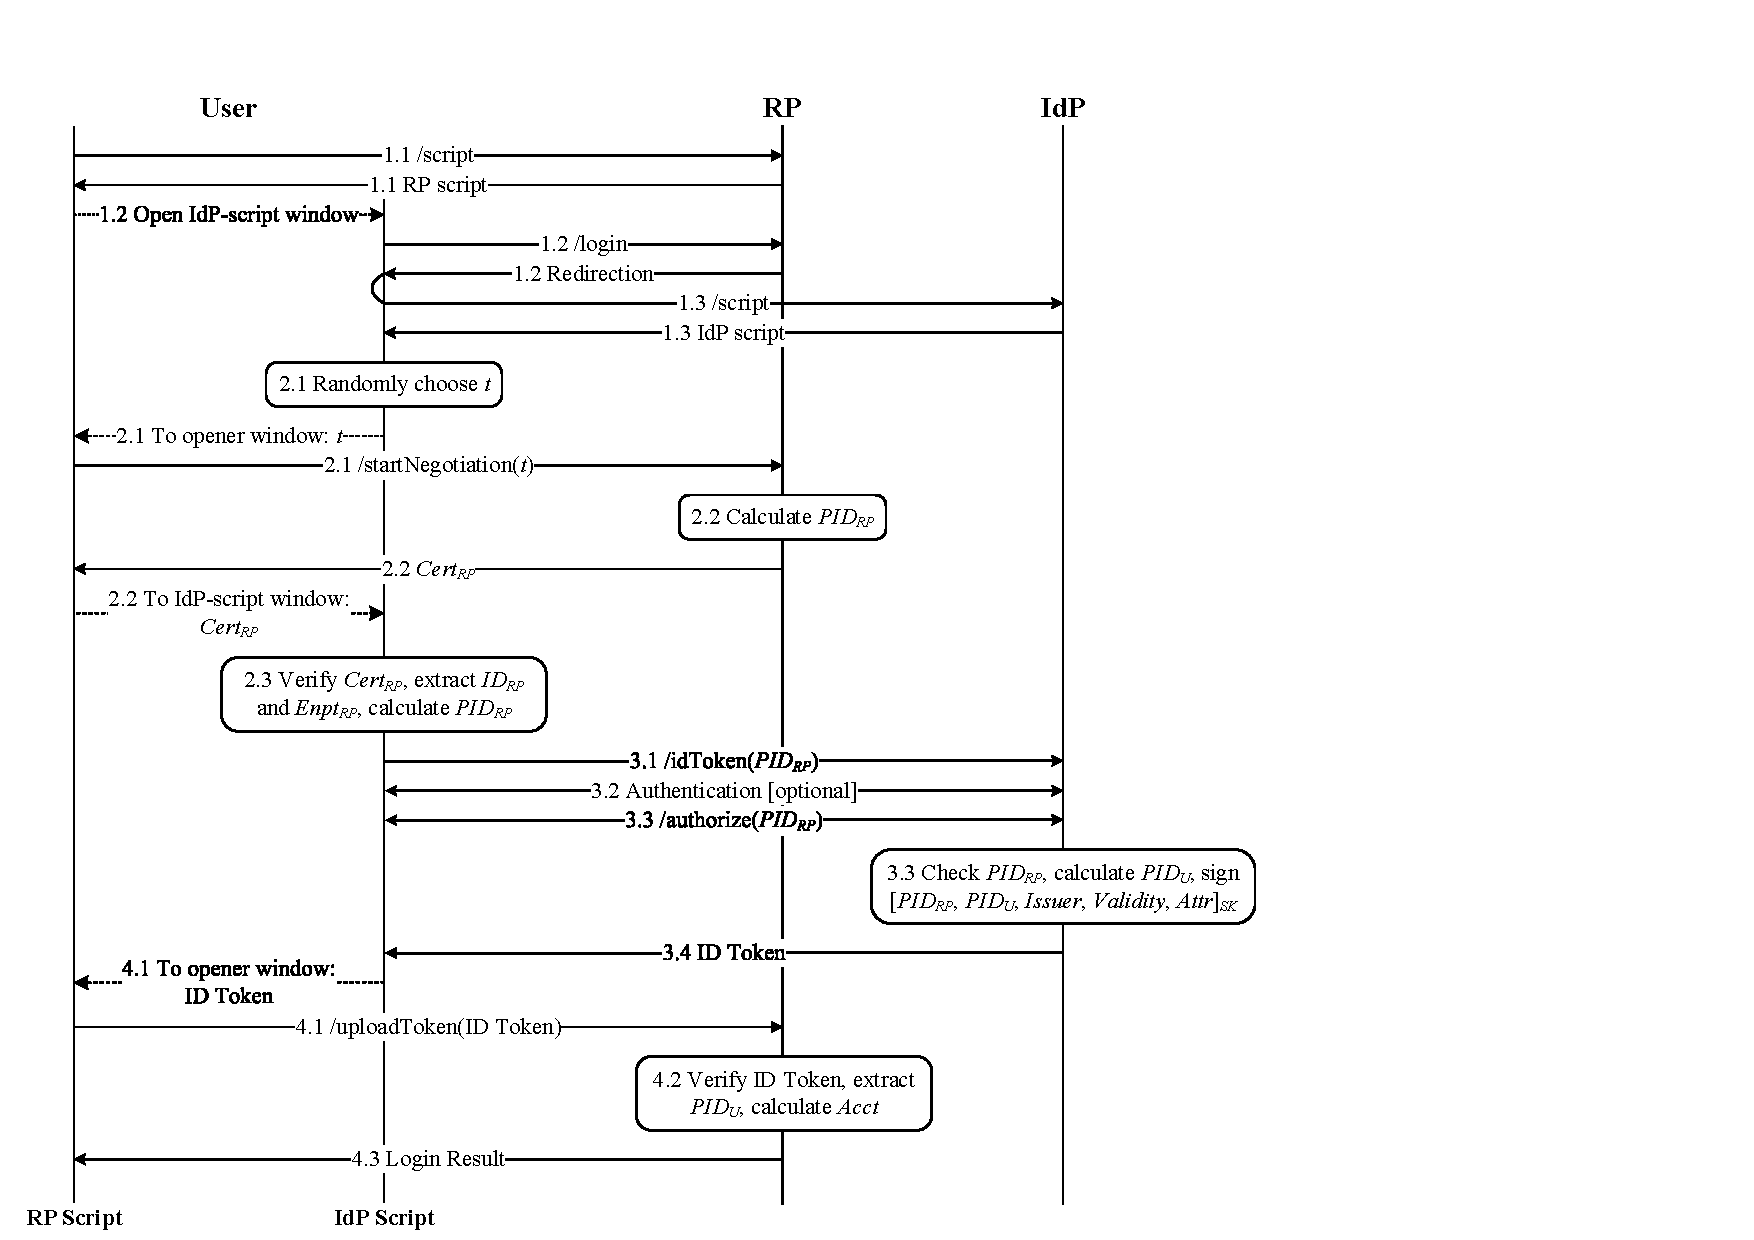
\includegraphics[height=0.575\textheight]{fig/process-js.pdf}
  \caption{The SSO login flow of UPPRESSO}
  \label{fig:process}
\end{figure*}


Finally,
    the browser downloads the RP script when visiting an RP,
     and this RP script opens a new window that downloads the IdP script.
We should prevent referer leakages when the IdP script is downloaded.
Generally, when a browser window visits another website not belonging to its opener's origin,
 the HTTP request to this website automatically carries a \verb+referer+ header (i.e., the opener's origin).
Such an HTTP header leaks the visited RP's domain to the IdP.
Fortunately, in UPPRESSO this newly-opened window is a \emph{redirection} from the RP to the IdP,
 but not a direct visit by browsers (Figure \ref{fig:process}, Steps 1.2-1.3).
This leakage is prevented by setting a \verb+referrer-policy=no-referrer+ header in the HTTP response from the RP,
 as it is redirected to the IdP.
So the HTTP request to download the IdP script carries no \verb+referer+ header.
This method is specified by W3C \cite{referer_policy} and widely supported.
We tested it in browsers such as Chrome, Safari, Edge, Opera and Firefox, and confirmed no referer leakage.




\subsection{The UPPRESSO Protocols}
\label{implementations}

\noindent \textbf{System Initialization.}
An IdP generates a key pair ($SK$, $PK$) to sign/verify identity tokens and RP certificates.
The IdP keeps $SK$ secret, and $PK$ is publicly known.


\vspace{1mm}
\noindent\textbf{RP Initial Registration.}
%Each RP launches an initial registration operation to finish configurations.
Each RP registers itself at the IdP to obtain $ID_{RP}$
 and its RP certificate $Cert_{RP}$ as follows:
\vspace{-\topsep}\begin{enumerate}
\setlength{\topsep}{0pt}
\setlength{\partopsep}{0pt}
\setlength{\itemsep}{0pt}
\setlength{\parsep}{0pt}
\setlength{\parskip}{0pt}
\item
An RP sends a registration request, including the endpoint to receive identity tokens
    and other information.
\item
The IdP randomly generates $r \in [1,n)$, until $ID_{RP} = [r]G$ is unique.
 %   but $r$ is kept unknown to the RP.
It signs $Cert_{RP} = [ID_{RP}, Enpt_{RP}, *]_{SK}$,
     where $[\cdot]_{SK}$ is a message signed using $SK$ and $*$ is supplementary information such as the RP's common name.
\item
The RP verifies $Cert_{RP}$ using $PK$,
    and accepts $ID_{RP}$ and $Cert_{RP}$ if they are valid.
\end{enumerate}


%\vspace{0.5mm}
\noindent\textbf{User Registration.}
Each user registers once at the IdP to set up a unique random identity $ID_U = u \in [1, n)$ and the corresponding credential. $ID_U$ is kept unknown to RPs.
%This is similar to the steps in existing SSO systems.


\vspace{1mm}
\noindent\textbf{SSO Login.} A login instance %is typically launched through a browser,
%when a user attempts to visit an RP. It
consists of four steps, namely script downloading, RP identity transformation,
identity-token generation, and $Acct$ calculation, as shown in Figure \ref{fig:process}.
In this figure,
    the IdP's operations are linked by a vertical line,
        so are the RP's.
Two vertical lines split the user operations into two groups (i.e., in two browser windows),
    one of which is to communicate with the IdP,
                 and the other is with the target RP.
Each solid horizontal line means some messages between the user and the IdP (or the RP),
            and each dotted line means a \verb+postMessage+ invocation between two scripts (or browser windows) within the browser.


\vspace{1mm}
\noindent 1. {\em Script Downloading.}
The browser downloads scripts from the visited RP and the IdP.
\vspace{-\topsep}
\begin{itemize}
\setlength{\topsep}{0pt}
\setlength{\partopsep}{0pt}
\setlength{\itemsep}{0pt}
\setlength{\parsep}{0pt}
\setlength{\parskip}{0pt}
\item[1.1]
When attempting to visit any protected resources at the RP,
    the user downloads the RP script.
\item[1.2]
The RP script opens a window in the browser to visit the login path at the RP, which is then redirected to the IdP.
\item[1.3]
The redirection to the IdP downloads the IdP script.
\end{itemize}



%\vspace{1mm}
\noindent 2. {\em RP Identity Transformation.}
The user and the RP negotiate $PID_{RP} = [t]{ID_{RP}}$.
\vspace{-\topsep}
\begin{itemize}
\setlength{\topsep}{0pt}
\setlength{\partopsep}{0pt}
\setlength{\itemsep}{0pt}
\setlength{\parsep}{0pt}
\setlength{\parskip}{0pt}
\item[2.1] The IdP script locally chooses a random number $t$ in $\mathbb{Z}_n$,
 and sends it to the RP script through \verb+postMessage+.
The RP script forwards $t$ to the RP.
\item[2.2] On receiving $t$,
the RP verifies $1 \leq t < n$ and %calculates $PID_{RP}$.
%To acknowledge the negotiation of $PID_{RP}$, The RP
 replies with $Cert_{RP}$, which is then transmitted from the RP script to the IdP script,
    with the scope of requested user attributes.  % through \verb+postMessage+.
\item[2.3] The IdP script locally verifies $Cert_{RP}$, extracts $ID_{RP}$ and $Enpt_{RP}$ from $Cert_{RP}$, and calculates $PID_{RP}=[t]{ID_{RP}}$.
%It then creates a random endpoint $PEnpt_{U}$ for this login instance,
 %   to receive identity tokens from the IdP.
    % as the RP endpoint required by IdP.我们已经修改了协议,IdP并不require什么

\end{itemize}


%\vspace{1mm}
\noindent 3. {\em Identity-Token Generation.}
The IdP calculates $PID_U = [ID_U]{PID_{RP}}$ and signs an identity token. % The processes are as follows.
\vspace{-\topsep}
\begin{itemize}
\setlength{\topsep}{0pt}
\setlength{\partopsep}{0pt}
\setlength{\itemsep}{0pt}
\setlength{\parsep}{0pt}
\setlength{\parskip}{0pt}
\item[3.1]
The IdP script sends an identity-token request for $PID_{RP}$ on behalf of the user. %and the user attributes.
 %by checking whether this user is authenticated by IdP.

\item[3.2] The IdP authenticates the user, if not authenticated yet.

\item [3.3]
The IdP script obtains the user's authorization for each requested attribute,
    and sends the scope of authorized attributes. % to the IdP.
\textcolor{blue}{Then, the IdP %checks that the received $PID_{RP}$ is a point on $\mathbb{E}$,
    calculates $PID_U = [ID_U]{PID_{RP}}$, % for the user,
and signs $[PID_{RP}, PID_U, Issuer, Validity, Attr]_{SK}$,}
 where $Issuer$ is the IdP's identity, $Validity$ indicates the validity period, and $Attr$ contains the authorized user attributes.
\item[3.4] The IdP replies with the identity token, to the IdP script.
\end{itemize}

%\vspace{1mm}
\noindent 4. {\em $Acct$ Calculation.}
The RP receives the identity token and allows the user to login.
\vspace{-\topsep}
\begin{itemize}
\setlength{\topsep}{0pt}
\setlength{\partopsep}{0pt}
\setlength{\itemsep}{0pt}
\setlength{\parsep}{0pt}
\setlength{\parskip}{0pt}
\item [4.1]
The IdP script forwards the identity token to the RP script,
    which sends it to the RP through $Enpt_{RP}$.
\item[4.2] The RP verifies the identity token, including the IdP's signature and its validity period.
Then, \textcolor{blue}{the RP extracts $PID_{RP}$ from the token, checks that it is equal to $[t]ID_{RP}$,}
and calculates $Acct = [t^{-1}]{PID_U}$.

\item [4.3] The RP allows the user to login as $Acct$.

\end{itemize}


If any verification or checking fails,
     this flow will be halted immediately.
For example, the user halts it
    on receiving invalid $Cert_{RP}$.
\textcolor{blue}{The IdP rejects an identity-token request Step 3.3, if the received $PID_{RP}$ is not a point on $\mathbb{E}$.
Or, the RP rejects an identity token in Step 4.2,
    if the signature is invalid or $PID_{RP}$ enclosed in it is not equal to $[t]ID_{RP}$.}



\subsection{Compatibility with OIDC}
\label{subsec:compatible}
First of all, UPPRESSO and OIDC work with COTS browsers.
Among the four steps of the login flow in UPPRESSO,
    \emph{script downloading} prepares the user agent.
The user agent is responsible for the communications between the IdP and the RP,
    which are implemented by HTTP redirections in OIDC.
On the contrary, in UPPRESSO the scripts hide $Enpt_{RP}$ from the IdP
%in UPPRESSO
 %   when sending the identity-token request,
  %      the script replaces $Enpt_{RP}$ with $PEnpt_{U}$,
    and forward the identity token to $Enpt_{RP}$ extracted from the RP certificate,
%    that to protect the identity token from being sent to adversaries. 这句话与Compatibility无关
so the IdP does not set \verb+redirect_uri+ in the HTTP responses. % of identity tokens.
Most operations of \emph{RP identity transformation} are conducted within browsers,
 while the RP only receives $t$ to prepare an RP pseudo-identity
  and responds with  $Cert_{RP}$.
%The calculation of $PID_{RP}$ is viewed as the operation to prepare an RP identity in OIDC,
The static $Cert_{RP}$ is viewed as a supplementary message to users.
%The operations in the $PID_{RP}$ registration are almost identical to those in the RP Dynamic Registration of OIDC \cite{DynamicRegistration},
   % except that
   % in OIDC the IdP assigns the RP's identity  while in UPPRESSO this (pseudo-)identity is generated by the registered entity.
%Besides, the $PID_{RP}$ registration has a validity period.
Thus, compared with the original OIDC protocol, in these two steps of UPPRESSO, the IdP's operations are simplified
    and an RP customizes its \emph{dynamic} pseudo-identity.

The operations of \emph{identity-token generation} and \emph{$Acct$ calculation},
    are actually \emph{identical} to those of OIDC,
    because (\emph{a}) the calculation of $PID_U$ is viewed as a method to generate PPIDs
        and (\emph{b}) the calculation of $Acct$ is viewed as a mapping from the user identity in tokens
                    to an account at the RP.

Finally,
    this compatibility is experimentally confirmed by our prototype implementation:
     only 23 lines of Java code in MITREid Connect \cite{MITREid}, an open-source OIDC system,
 are modified
    to build an IdP of UPPRESSO (see Section \ref{subsec:proto-imple}).
%It will help the adoption and deployment of UPPRESSO.

